\section{Příklad 4}
% Jako parametr zadejte skupinu (A-H)
\ctvrtyZadani{A}

\subsection{Řešení}

V tomto příkladě máme za úkol vypočítat amplitudu a fázi napětí na kondenzátoru $C_2$ v obvodu se 
střídavým proudem, a to za využití metody smyčkových proudů. 

Při výpočtu budeme využívat komplexních impedancí kondenzátorů a cívek, které si můžeme pro začátek vypočítat:

$$ Z_{C1} = -\frac{j}{\omega C_1} = -\frac{j}{2 \pi f C_1} \doteq -11,3682j \: \Omega $$

$$ Z_{C2} = -\frac{j}{2 \pi f C_2} \doteq -21,6537j \: \Omega $$

$$ Z_{L1} = j \omega L_1 = 2 j \pi f L_1 \doteq 52,7788j \: \Omega $$

$$ Z_{L2} = 2 j \pi f L_2 \doteq 43,9823j \: \Omega $$

Následně si do obvodu zaznačíme směrové šipky smyčkových proudů $I_a$, $I_b$ a $I_c$. 

\begin{figure}[H]
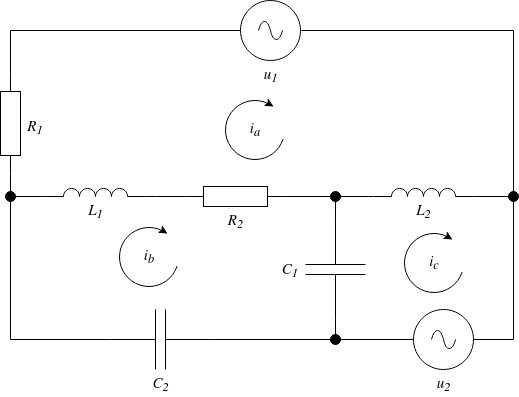
\includegraphics[scale=0.5]{Pr4/step1.png}
\centering
\caption{Označení smyčkových proudů v obvodu}
\end{figure}

Nyní si pro každou smyčku sestavíme rovnici na základě druhého Kirchoffova zákona: 

$$ Smyčka \: A: \: i_aR_1 + u_1 + (i_a - i_c)Z_{L2} + (i_a - i_b)R_2 + (i_a - i_b)Z_{L1} = 0 $$

$$ Smyčka \: B: \: (i_b - i_c)Z_{C1} + i_bZ_{C2} + (i_b - i_a)Z_{L1} + (i_b - i_a)R_2 = 0 $$

$$ Smyčka \: C: \: (i_c - i_a)Z_{L2} + u_2 + (i_c - i_b)Z_{C1} = 0 $$

Tuto soustavu rovnic přepíšeme do matice:

$$ \left (
\begin{array}{ccc|c}
	R_1 + Z_{L2} + R_2 + Z_{L1} & -R_2 - Z_{L1} & -Z_{L2} & - u_1 \\
	-R_2 - Z_{L1} & Z_{C1} + Z_{C2} + Z_{L1} + R_2 & -Z_{C1} & 0 \\
	-Z_{L2} & -Z_{C1} & Z_{L2} + Z_{C1} & - u_2
\end{array}
\right) $$

Do této matice dosadíme konkrétní hodnoty, které jsme si vypočítali výše, a vyřešíme např. eliminační metodou. Pro přehlednost zde nebudu celý výpočet uvádět. Zajímá nás hodnota proudu $i_b$, jelikož kondenzátorem $C_2$ teče právě proud $i_b$. 

Po vyřešení soustavy rovnic nám vyjde, že $i_b \doteq 0,05676 + 0.3126 j \: A$. Komplexní hodnotu napětí určíme jednoduše, podle následnující rovnice: 

$$ u_{C2} = i_b Z_{C2} \doteq - 6.7696 + 1.2291j \: V $$

Amplitudu napětí na kondenzátoru $C_2$ pak určíme jako velikost tohoto komplexního čísla:

$$ |u_{C2}| = |- 6.7696 + 1.2291j| \doteq 6,8803 \: V $$

Nakonec, fázový posun $\varphi_{C2}$ bude odpovídat fázi komplexního čísla $u_{C2}$:

$$ \varphi_{C2} = arg(6.7696 - 1.2291j) \doteq 169.7093 ^\circ $$
